\begin{figure}[htpb]
	\centering\capstart{}
	\subfloat[\(\Re{\pixel{\mathcal{EG}}}\)]{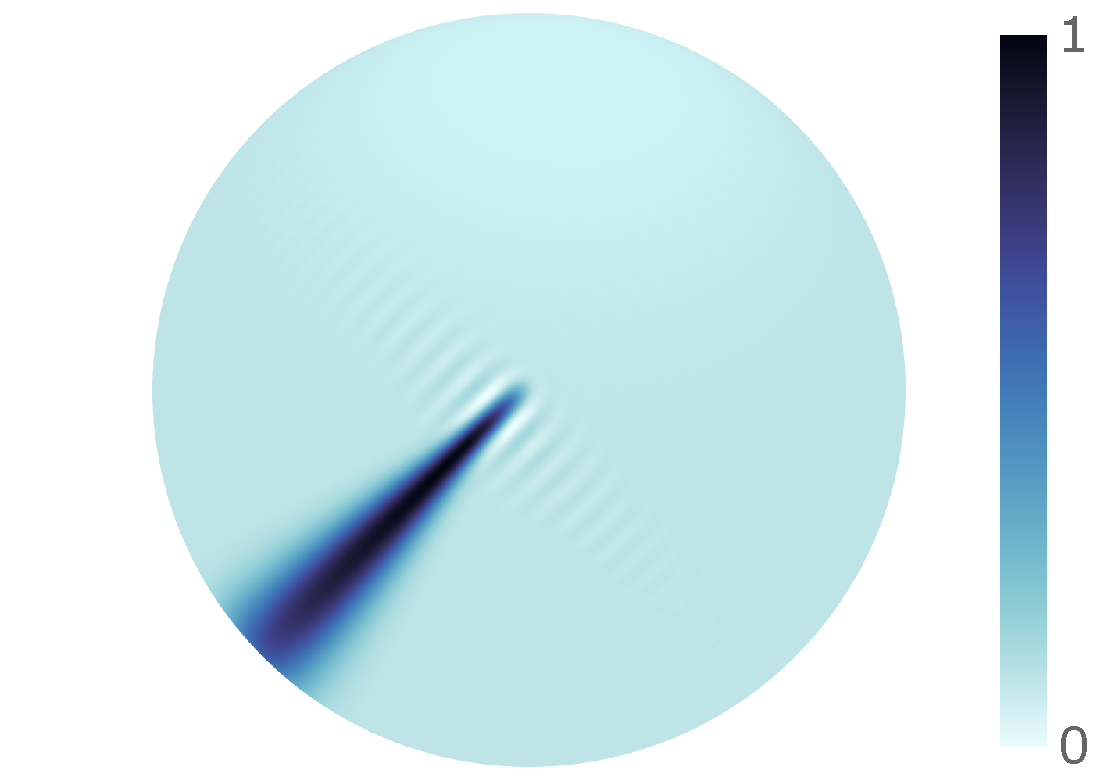
\includegraphics[trim={23 7 3 6},clip,width=.5\textwidth]{elongated_gaussian_1tsig_1psig10_L128_res512_real_norm.pdf}}
	\hfill
	\subfloat[\(\Re{\pixel{(\translation{\omega'}\mathcal{EG})}}\)]{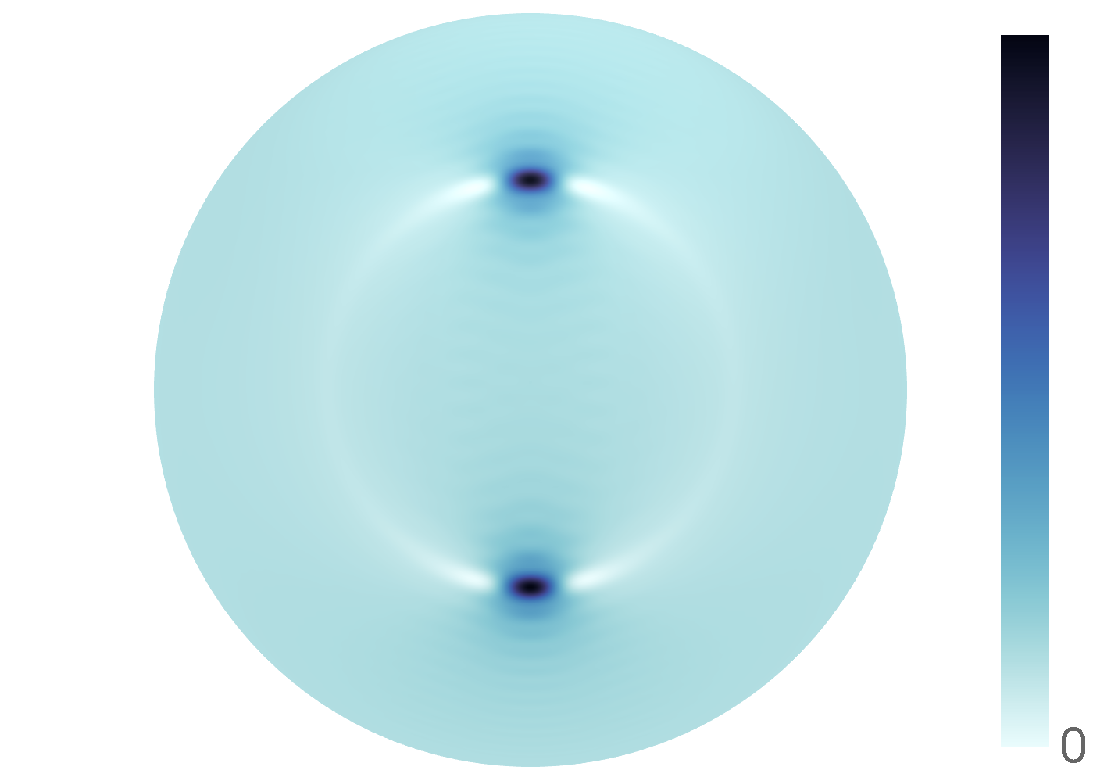
\includegraphics[trim={23 7 3 6},clip,width=.5\textwidth]{elongated_gaussian_1tsig_1psig10_L128_translate_alpha3pi4_beta1pi8_res512_real_norm.pdf}}
	\caption[
		An elongated Gaussian on the north pole and then translated
	]{
		Panel (a) presents the elongated Gaussian on the north pole (bandlimited at \(L=128\)) --- where the central bar in the plot extends over half of the sphere.
		The elongated Gaussian is then translated to some \(\omega'=(\theta',\phi')\), as shown in panel (b).
		The even azimuthal symmetry in the initial kernel definition results into the two localised components at \(\phi'\) and \(-\phi'\) under translation.
		The colour is between zero and one, reflecting the scaled intensity of the field.
	}\label{fig:chapter3_elongated_gaussian}
\end{figure}
